\section{Kotne funkcije}

\begin{frame}
    \sectionpage
\end{frame}

\begin{frame}
    \tableofcontents[currentsection, hideothersubsections]
\end{frame}

    \subsection{Kotne funkcije poljubnih kotov}

        \begin{frame}
            \frametitle{Stopinje in radiani}

            \begin{alertblock}{Radian}
                Loku na krožnici, ki je enako dolg kot polmer krožnice, pripada središčni kot, velik $1 \ \textrm{radian}$.
                $$ 1 \ \textrm{rad}=\frac{180^\circ}{\pi}\doteq 57,3^\circ$$
            \end{alertblock}

            \begin{exampleblock}{Pretvorba med stopinjami in radiani}
                Naj bo $\varphi$ kot podan v radianih, $\phi$ pa njemu pripadajoči kot podan v stopinjah. Potem velja:
                $$ \varphi = \frac{\pi}{180^\circ}\phi$$
                in 
                $$ \phi = \frac{180^\circ}{\pi} \varphi.$$
            \end{exampleblock}
        \end{frame}

        
        \begin{frame}
            \frametitle{Kotne funkcije v pravokotnem trikotniku}

            % \begin{figure}
            %     \begin{tikzpicture}
            %         % \clip (0,0) rectangle (14.000000,10.000000);
            %         {\footnotesize
                    
            %         % Marking point C by circle
            %         \draw [line width=0.016cm] (2.300000,3.100000) circle (0.040000);%
            %         \draw (2.300000,3.100000) node [anchor=south] { $C$ };%
                    
            %         % Marking point A by circle
            %         \draw [line width=0.016cm] (1.500000,1.500000) circle (0.040000);%
            %         \draw (1.500000,1.500000) node [anchor=north] { $A$ };%
                    
            %         % Marking point B by circle
            %         \draw [line width=0.016cm] (5.500000,1.500000) circle (0.040000);%
            %         \draw (5.500000,1.500000) node [anchor=north] { $B$ };%
                    
            %         % Drawing segment A C
            %         \draw [line width=0.016cm] (1.517889,1.535777) -- (2.282111,3.064223);%
                    
            %         % Drawing segment A B
            %         \draw [line width=0.016cm] (1.540000,1.500000) -- (5.460000,1.500000);%
                    
            %         % Drawing segment B C
            %         \draw [line width=0.016cm] (5.464223,1.517889) -- (2.335777,3.082111);%
                    
            %         % Marking point \alpha
            %         \draw (1.800000,1.500000) node [anchor=south] { $\alpha$ };%
                    
            %         % Marking point \frac{\pi}{2}
            %         \draw (2.400000,3.100000) node [anchor=north] { $\frac{\pi}{2}$ };%
                    
            %         % Marking point h
            %         \draw (3.500000,1.500000) node [anchor=north] { $h$ };%
                    
            %         % Marking point pk
            %         \draw (1.900000,2.300000) node [anchor=east] { $pk$ };%
                    
            %         % Marking point nk
            %         \draw (3.800000,2.300000) node [anchor=south west] { $nk$ };%
            %         }
            %     \end{tikzpicture}                    
            % \end{figure}

            \begin{columns}
                \column{0.48\textwidth}
                        \textbf{Sinus} kota $\alpha$ je količnik med kotu $\alpha$ nasprotno kateto in hipotenuzo: $$\sin\alpha = \frac{\textrm{nasprotna kateta}}{\textrm{hipotenuza}}.$$
                        \textbf{Kosinus} kota $\alpha$ je količnik med kotu $\alpha$ priležno kateto in hipotenuzo: $$\cos\alpha = \frac{\textrm{priležna kateta}}{\textrm{hipotenuza}}.$$
                        \textbf{Tangens} kota $\alpha$ je količnik med kotu $\alpha$ nasprotno kateto in priležno kateto: $$\tan\alpha = \frac{\textrm{nasprotna kateta}}{\textrm{priležna kateta}}.$$

                \column{0.48\textwidth}
                    \begin{figure}
                        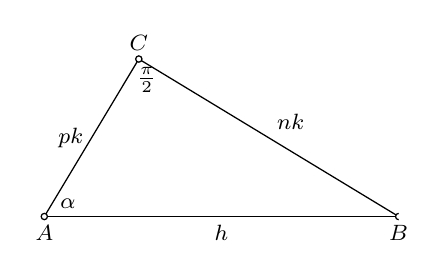
\begin{tikzpicture}
                            % \clip (0,0) rectangle (14.000000,10.000000);
                            {\footnotesize
                            
                            % Marking point C by circle
                            \draw [line width=0.016cm] (2.700000,3.500000) circle (0.040000);%
                            \draw (2.700000,3.500000) node [anchor=south] { $C$ };%
                            
                            % Marking point A by circle
                            \draw [line width=0.016cm] (1.500000,1.500000) circle (0.040000);%
                            \draw (1.500000,1.500000) node [anchor=north] { $A$ };%
                            
                            % Marking point B by circle
                            \draw [line width=0.016cm] (6.000000,1.540000) arc (90:269:0.040000 and 0.040000) -- (6.000000,1.460000);%
                            \draw (6.000000,1.500000) node [anchor=north] { $B$ };%
                            
                            % Drawing segment A C
                            \draw [line width=0.016cm] (1.520580,1.534300) -- (2.679420,3.465700);%
                            
                            % Drawing segment A B
                            \draw [line width=0.016cm] (1.540000,1.500000) -- (5.960000,1.500000);%
                            
                            % Drawing segment B C
                            \draw [line width=0.016cm] (5.965792,1.520732) -- (2.734208,3.479268);%
                            
                            % Marking point \alpha
                            \draw (1.800000,1.500000) node [anchor=south] { $\alpha$ };%
                            
                            % Marking point \frac{\pi}{2}
                            \draw (2.800000,3.500000) node [anchor=north] { $\frac{\pi}{2}$ };%
                            
                            % Marking point h
                            \draw (3.750000,1.500000) node [anchor=north] { $h$ };%
                            
                            % Marking point pk
                            \draw (2.100000,2.500000) node [anchor=east] { $pk$ };%
                            
                            % Marking point nk
                            \draw (4.350000,2.500000) node [anchor=south west] { $nk$ };%
                            }
                            \end{tikzpicture}
                        \end{figure}
                        ~\\
                        ~\\
                        \textbf{Kotangens} kota $\alpha$ je količnik med kotu $\alpha$ priležno kateto in nasprotno kateto: $$\cot\alpha = \frac{\textrm{priležna kateta}}{\textrm{nasprotna kateta}}.$$
            \end{columns}

        \end{frame}


        \begin{frame}
            \frametitle{Kotne funkcije komplementarnih kotov}

            \begin{alertblock}{}
                Sinus kota je enak kosinusu komplementarnega kota in obratno.
                $$ \cos{\frac{\pi}{2}-\alpha} = \sin\alpha $$
                $$ \sin{\frac{\pi}{2}-\alpha} = \cos\alpha $$
            \end{alertblock}

            \begin{alertblock}{}
                Tangens kota je enak kotangensu komplementarnega kota in obratno.
                $$ \tan{\frac{\pi}{2}-\alpha} = \cot\alpha $$
                $$ \cot{\frac{\pi}{2}-\alpha} = \tan\alpha $$
            \end{alertblock}
        \end{frame}
        

        \begin{frame}
            \frametitle{Kotne funkcije v enotskem krogu}

            \begin{figure}
                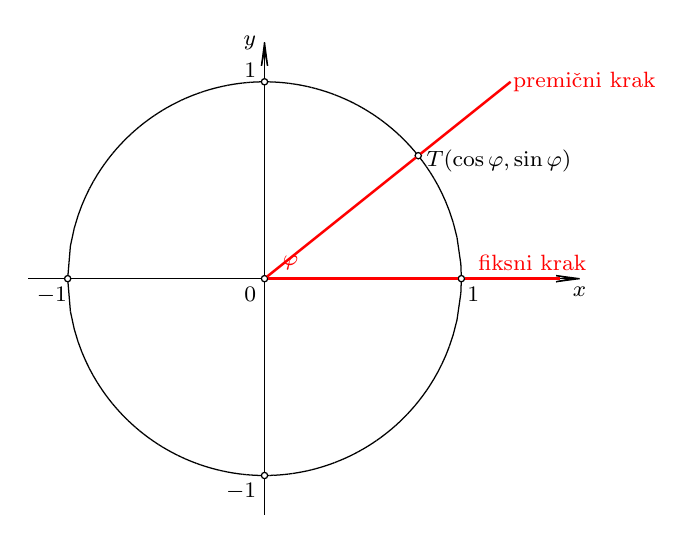
\begin{tikzpicture}
                    % \clip (0,0) rectangle (14.000000,10.000000);
                    {\footnotesize
                    
                    % Drawing 2D Cartesian system
                    \draw [line width=0.016cm] (3.000000,3.000000) circle (0.040000);%
                    \draw (3.000000,3.000000) node [anchor=north east] { $0$ };%
                    \draw [line width=0.016cm] (5.500000,3.000000) circle (0.040000);%
                    \draw (5.650000,3.000000) node [anchor=north] { $1$ };%
                    \draw [line width=0.016cm] (0.500000,3.000000) circle (0.040000);%
                    \draw (0.300000,3.000000) node [anchor=north] { $-1$ };%
                    \draw [line width=0.016cm] (3.000000,5.500000) circle (0.040000);%
                    \draw (3.000000,5.650000) node [anchor=east] { $1$ };%
                    \draw [line width=0.016cm] (3.000000,0.500000) circle (0.040000);%
                    \draw (3.000000,0.300000) node [anchor=east] { $-1$ };%
                    \draw (7.000000,3.000000) node [anchor=north] { $x$ };%
                    \draw (3.000000,6.000000) node [anchor=east] { $y$ };%
                    \draw [line width=0.016cm] (0.000000,3.000000) -- (0.460000,3.000000);%
                    \draw [line width=0.016cm] (0.540000,3.000000) -- (2.960000,3.000000);%
                    \draw [line width=0.016cm] (3.040000,3.000000) -- (5.460000,3.000000);%
                    \draw [line width=0.016cm] (5.540000,3.000000) -- (7.000000,3.000000);%
                    \draw [line width=0.016cm] (6.702567,3.039158) -- (7.000000,3.000000);%
                    \draw [line width=0.016cm] (6.702567,3.039158) -- (6.900000,3.000000);%
                    \draw [line width=0.016cm] (6.702567,2.960842) -- (7.000000,3.000000);%
                    \draw [line width=0.016cm] (6.702567,2.960842) -- (6.900000,3.000000);%
                    \draw [line width=0.016cm] (3.000000,0.000000) -- (3.000000,0.460000);%
                    \draw [line width=0.016cm] (3.000000,0.540000) -- (3.000000,2.960000);%
                    \draw [line width=0.016cm] (3.000000,3.040000) -- (3.000000,5.460000);%
                    \draw [line width=0.016cm] (3.000000,5.540000) -- (3.000000,6.000000);%
                    \draw [line width=0.016cm] (2.960842,5.702567) -- (3.000000,6.000000);%
                    \draw [line width=0.016cm] (2.960842,5.702567) -- (3.000000,5.900000);%
                    \draw [line width=0.016cm] (3.039158,5.702567) -- (3.000000,6.000000);%
                    \draw [line width=0.016cm] (3.039158,5.702567) -- (3.000000,5.900000);%
                    
                    % Drawing 2D ang conic k
                    \draw [line width=0.016cm] (0.503333,3.039861) -- (0.517361,3.207609);%
                    \draw [line width=0.016cm] (0.517361,3.207609) -- (0.534722,3.415217);%
                    \draw [line width=0.016cm] (0.503333,2.960139) -- (0.517361,2.792391);%
                    \draw [line width=0.016cm] (0.517361,2.792391) -- (0.534722,2.584783);%
                    \draw [line width=0.016cm] (0.534722,3.415217) -- (0.583333,3.640095);%
                    \draw [line width=0.016cm] (0.534722,2.584783) -- (0.583333,2.359905);%
                    \draw [line width=0.016cm] (0.583333,3.640095) -- (0.631944,3.801444);%
                    \draw [line width=0.016cm] (0.583333,2.359905) -- (0.631944,2.198556);%
                    \draw [line width=0.016cm] (0.631944,3.801444) -- (0.680556,3.932833);%
                    \draw [line width=0.016cm] (0.631944,2.198556) -- (0.680556,2.067167);%
                    \draw [line width=0.016cm] (0.680556,3.932833) -- (0.729167,4.045618);%
                    \draw [line width=0.016cm] (0.680556,2.067167) -- (0.729167,1.954382);%
                    \draw [line width=0.016cm] (0.729167,4.045618) -- (0.777778,4.145307);%
                    \draw [line width=0.016cm] (0.729167,1.954382) -- (0.777778,1.854693);%
                    \draw [line width=0.016cm] (0.777778,4.145307) -- (0.826389,4.235077);%
                    \draw [line width=0.016cm] (0.777778,1.854693) -- (0.826389,1.764923);%
                    \draw [line width=0.016cm] (0.826389,4.235077) -- (0.875000,4.316957);%
                    \draw [line width=0.016cm] (0.826389,1.764923) -- (0.875000,1.683043);%
                    \draw [line width=0.016cm] (0.875000,4.316957) -- (0.923611,4.392339);%
                    \draw [line width=0.016cm] (0.875000,1.683043) -- (0.923611,1.607661);%
                    \draw [line width=0.016cm] (0.923611,4.392339) -- (0.972222,4.462230);%
                    \draw [line width=0.016cm] (0.923611,1.607661) -- (0.972222,1.537770);%
                    \draw [line width=0.016cm] (0.972222,4.462230) -- (1.020833,4.527383);%
                    \draw [line width=0.016cm] (0.972222,1.537770) -- (1.020833,1.472617);%
                    \draw [line width=0.016cm] (1.020833,4.527383) -- (1.069444,4.588381);%
                    \draw [line width=0.016cm] (1.020833,1.472617) -- (1.069444,1.411619);%
                    \draw [line width=0.016cm] (1.069444,4.588381) -- (1.118056,4.645687);%
                    \draw [line width=0.016cm] (1.069444,1.411619) -- (1.118056,1.354313);%
                    \draw [line width=0.016cm] (1.118056,4.645687) -- (1.166667,4.699673);%
                    \draw [line width=0.016cm] (1.118056,1.354313) -- (1.166667,1.300327);%
                    \draw [line width=0.016cm] (1.166667,4.699673) -- (1.215278,4.750647);%
                    \draw [line width=0.016cm] (1.166667,1.300327) -- (1.215278,1.249353);%
                    \draw [line width=0.016cm] (1.215278,4.750647) -- (1.263889,4.798866);%
                    \draw [line width=0.016cm] (1.215278,1.249353) -- (1.263889,1.201134);%
                    \draw [line width=0.016cm] (1.263889,4.798866) -- (1.312500,4.844544);%
                    \draw [line width=0.016cm] (1.263889,1.201134) -- (1.312500,1.155456);%
                    \draw [line width=0.016cm] (1.312500,4.844544) -- (1.361111,4.887867);%
                    \draw [line width=0.016cm] (1.312500,1.155456) -- (1.361111,1.112133);%
                    \draw [line width=0.016cm] (1.361111,4.887867) -- (1.409722,4.928994);%
                    \draw [line width=0.016cm] (1.361111,1.112133) -- (1.409722,1.071006);%
                    \draw [line width=0.016cm] (1.409722,4.928994) -- (1.458333,4.968061);%
                    \draw [line width=0.016cm] (1.409722,1.071006) -- (1.458333,1.031939);%
                    \draw [line width=0.016cm] (1.458333,4.968061) -- (1.506944,5.005190);%
                    \draw [line width=0.016cm] (1.458333,1.031939) -- (1.506944,0.994810);%
                    \draw [line width=0.016cm] (1.506944,5.005190) -- (1.555556,5.040485);%
                    \draw [line width=0.016cm] (1.506944,0.994810) -- (1.555556,0.959515);%
                    \draw [line width=0.016cm] (1.555556,5.040485) -- (1.604167,5.074042);%
                    \draw [line width=0.016cm] (1.555556,0.959515) -- (1.604167,0.925958);%
                    \draw [line width=0.016cm] (1.604167,5.074042) -- (1.652778,5.105942);%
                    \draw [line width=0.016cm] (1.604167,0.925958) -- (1.652778,0.894058);%
                    \draw [line width=0.016cm] (1.652778,5.105942) -- (1.701389,5.136261);%
                    \draw [line width=0.016cm] (1.652778,0.894058) -- (1.701389,0.863739);%
                    \draw [line width=0.016cm] (1.701389,5.136261) -- (1.750000,5.165064);%
                    \draw [line width=0.016cm] (1.701389,0.863739) -- (1.750000,0.834936);%
                    \draw [line width=0.016cm] (1.750000,5.165064) -- (1.798611,5.192411);%
                    \draw [line width=0.016cm] (1.750000,0.834936) -- (1.798611,0.807589);%
                    \draw [line width=0.016cm] (1.798611,5.192411) -- (1.847222,5.218356);%
                    \draw [line width=0.016cm] (1.798611,0.807589) -- (1.847222,0.781644);%
                    \draw [line width=0.016cm] (1.847222,5.218356) -- (1.895833,5.242948);%
                    \draw [line width=0.016cm] (1.847222,0.781644) -- (1.895833,0.757052);%
                    \draw [line width=0.016cm] (1.895833,5.242948) -- (1.944444,5.266231);%
                    \draw [line width=0.016cm] (1.895833,0.757052) -- (1.944444,0.733769);%
                    \draw [line width=0.016cm] (1.944444,5.266231) -- (1.993056,5.288244);%
                    \draw [line width=0.016cm] (1.944444,0.733769) -- (1.993056,0.711756);%
                    \draw [line width=0.016cm] (1.993056,5.288244) -- (2.041667,5.309025);%
                    \draw [line width=0.016cm] (1.993056,0.711756) -- (2.041667,0.690975);%
                    \draw [line width=0.016cm] (2.041667,5.309025) -- (2.090278,5.328606);%
                    \draw [line width=0.016cm] (2.041667,0.690975) -- (2.090278,0.671394);%
                    \draw [line width=0.016cm] (2.090278,5.328606) -- (2.138889,5.347017);%
                    \draw [line width=0.016cm] (2.090278,0.671394) -- (2.138889,0.652983);%
                    \draw [line width=0.016cm] (2.138889,5.347017) -- (2.187500,5.364285);%
                    \draw [line width=0.016cm] (2.138889,0.652983) -- (2.187500,0.635715);%
                    \draw [line width=0.016cm] (2.187500,5.364285) -- (2.236111,5.380436);%
                    \draw [line width=0.016cm] (2.187500,0.635715) -- (2.236111,0.619564);%
                    \draw [line width=0.016cm] (2.236111,5.380436) -- (2.284722,5.395491);%
                    \draw [line width=0.016cm] (2.236111,0.619564) -- (2.284722,0.604509);%
                    \draw [line width=0.016cm] (2.284722,5.395491) -- (2.333333,5.409472);%
                    \draw [line width=0.016cm] (2.284722,0.604509) -- (2.333333,0.590528);%
                    \draw [line width=0.016cm] (2.333333,5.409472) -- (2.381944,5.422397);%
                    \draw [line width=0.016cm] (2.333333,0.590528) -- (2.381944,0.577603);%
                    \draw [line width=0.016cm] (2.381944,5.422397) -- (2.430556,5.434283);%
                    \draw [line width=0.016cm] (2.381944,0.577603) -- (2.430556,0.565717);%
                    \draw [line width=0.016cm] (2.430556,5.434283) -- (2.479167,5.445145);%
                    \draw [line width=0.016cm] (2.430556,0.565717) -- (2.479167,0.554855);%
                    \draw [line width=0.016cm] (2.479167,5.445145) -- (2.527778,5.454996);%
                    \draw [line width=0.016cm] (2.479167,0.554855) -- (2.527778,0.545004);%
                    \draw [line width=0.016cm] (2.527778,5.454996) -- (2.576389,5.463849);%
                    \draw [line width=0.016cm] (2.527778,0.545004) -- (2.576389,0.536151);%
                    \draw [line width=0.016cm] (2.576389,5.463849) -- (2.625000,5.471715);%
                    \draw [line width=0.016cm] (2.576389,0.536151) -- (2.625000,0.528285);%
                    \draw [line width=0.016cm] (2.625000,5.471715) -- (2.673611,5.478602);%
                    \draw [line width=0.016cm] (2.625000,0.528285) -- (2.673611,0.521398);%
                    \draw [line width=0.016cm] (2.673611,5.478602) -- (2.722222,5.484520);%
                    \draw [line width=0.016cm] (2.673611,0.521398) -- (2.722222,0.515480);%
                    \draw [line width=0.016cm] (2.722222,5.484520) -- (2.770833,5.489474);%
                    \draw [line width=0.016cm] (2.722222,0.515480) -- (2.770833,0.510526);%
                    \draw [line width=0.016cm] (2.770833,5.489474) -- (2.819444,5.493471);%
                    \draw [line width=0.016cm] (2.770833,0.510526) -- (2.819444,0.506529);%
                    \draw [line width=0.016cm] (2.819444,5.493471) -- (2.868056,5.496516);%
                    \draw [line width=0.016cm] (2.819444,0.506529) -- (2.868056,0.503484);%
                    \draw [line width=0.016cm] (2.868056,5.496516) -- (2.916667,5.498611);%
                    \draw [line width=0.016cm] (2.868056,0.503484) -- (2.916667,0.501389);%
                    \draw [line width=0.016cm] (2.916667,5.498611) -- (2.960002,5.499634);%
                    \draw [line width=0.016cm] (2.916667,0.501389) -- (2.960002,0.500366);%
                    \draw [line width=0.016cm] (3.039998,5.499562) -- (3.062500,5.499219);%
                    \draw [line width=0.016cm] (3.039998,0.500438) -- (3.062500,0.500781);%
                    \draw [line width=0.016cm] (3.062500,5.499219) -- (3.111111,5.497530);%
                    \draw [line width=0.016cm] (3.062500,0.500781) -- (3.111111,0.502470);%
                    \draw [line width=0.016cm] (3.111111,5.497530) -- (3.159722,5.494893);%
                    \draw [line width=0.016cm] (3.111111,0.502470) -- (3.159722,0.505107);%
                    \draw [line width=0.016cm] (3.159722,5.494893) -- (3.208333,5.491304);%
                    \draw [line width=0.016cm] (3.159722,0.505107) -- (3.208333,0.508696);%
                    \draw [line width=0.016cm] (3.208333,5.491304) -- (3.256944,5.486761);%
                    \draw [line width=0.016cm] (3.208333,0.508696) -- (3.256944,0.513239);%
                    \draw [line width=0.016cm] (3.256944,5.486761) -- (3.305556,5.481257);%
                    \draw [line width=0.016cm] (3.256944,0.513239) -- (3.305556,0.518743);%
                    \draw [line width=0.016cm] (3.305556,5.481257) -- (3.354167,5.474786);%
                    \draw [line width=0.016cm] (3.305556,0.518743) -- (3.354167,0.525214);%
                    \draw [line width=0.016cm] (3.354167,5.474786) -- (3.402778,5.467341);%
                    \draw [line width=0.016cm] (3.354167,0.525214) -- (3.402778,0.532659);%
                    \draw [line width=0.016cm] (3.402778,5.467341) -- (3.451389,5.458912);%
                    \draw [line width=0.016cm] (3.402778,0.532659) -- (3.451389,0.541088);%
                    \draw [line width=0.016cm] (3.451389,5.458912) -- (3.500000,5.449490);%
                    \draw [line width=0.016cm] (3.451389,0.541088) -- (3.500000,0.550510);%
                    \draw [line width=0.016cm] (3.500000,5.449490) -- (3.548611,5.439062);%
                    \draw [line width=0.016cm] (3.500000,0.550510) -- (3.548611,0.560938);%
                    \draw [line width=0.016cm] (3.548611,5.439062) -- (3.597222,5.427617);%
                    \draw [line width=0.016cm] (3.548611,0.560938) -- (3.597222,0.572383);%
                    \draw [line width=0.016cm] (3.597222,5.427617) -- (3.645833,5.415140);%
                    \draw [line width=0.016cm] (3.597222,0.572383) -- (3.645833,0.584860);%
                    \draw [line width=0.016cm] (3.645833,5.415140) -- (3.694444,5.401613);%
                    \draw [line width=0.016cm] (3.645833,0.584860) -- (3.694444,0.598387);%
                    \draw [line width=0.016cm] (3.694444,5.401613) -- (3.743056,5.387021);%
                    \draw [line width=0.016cm] (3.694444,0.598387) -- (3.743056,0.612979);%
                    \draw [line width=0.016cm] (3.743056,5.387021) -- (3.791667,5.371342);%
                    \draw [line width=0.016cm] (3.743056,0.612979) -- (3.791667,0.628658);%
                    \draw [line width=0.016cm] (3.791667,5.371342) -- (3.840278,5.354556);%
                    \draw [line width=0.016cm] (3.791667,0.628658) -- (3.840278,0.645444);%
                    \draw [line width=0.016cm] (3.840278,5.354556) -- (3.888889,5.336638);%
                    \draw [line width=0.016cm] (3.840278,0.645444) -- (3.888889,0.663362);%
                    \draw [line width=0.016cm] (3.888889,5.336638) -- (3.937500,5.317562);%
                    \draw [line width=0.016cm] (3.888889,0.663362) -- (3.937500,0.682438);%
                    \draw [line width=0.016cm] (3.937500,5.317562) -- (3.986111,5.297299);%
                    \draw [line width=0.016cm] (3.937500,0.682438) -- (3.986111,0.702701);%
                    \draw [line width=0.016cm] (3.986111,5.297299) -- (4.034722,5.275819);%
                    \draw [line width=0.016cm] (3.986111,0.702701) -- (4.034722,0.724181);%
                    \draw [line width=0.016cm] (4.034722,5.275819) -- (4.083333,5.253084);%
                    \draw [line width=0.016cm] (4.034722,0.724181) -- (4.083333,0.746916);%
                    \draw [line width=0.016cm] (4.083333,5.253084) -- (4.131944,5.229058);%
                    \draw [line width=0.016cm] (4.083333,0.746916) -- (4.131944,0.770942);%
                    \draw [line width=0.016cm] (4.131944,5.229058) -- (4.180556,5.203699);%
                    \draw [line width=0.016cm] (4.131944,0.770942) -- (4.180556,0.796301);%
                    \draw [line width=0.016cm] (4.180556,5.203699) -- (4.229167,5.176959);%
                    \draw [line width=0.016cm] (4.180556,0.796301) -- (4.229167,0.823041);%
                    \draw [line width=0.016cm] (4.229167,5.176959) -- (4.277778,5.148787);%
                    \draw [line width=0.016cm] (4.229167,0.823041) -- (4.277778,0.851213);%
                    \draw [line width=0.016cm] (4.277778,5.148787) -- (4.326389,5.119125);%
                    \draw [line width=0.016cm] (4.277778,0.851213) -- (4.326389,0.880875);%
                    \draw [line width=0.016cm] (4.326389,5.119125) -- (4.375000,5.087912);%
                    \draw [line width=0.016cm] (4.326389,0.880875) -- (4.375000,0.912088);%
                    \draw [line width=0.016cm] (4.375000,5.087912) -- (4.423611,5.055075);%
                    \draw [line width=0.016cm] (4.375000,0.912088) -- (4.423611,0.944925);%
                    \draw [line width=0.016cm] (4.423611,5.055075) -- (4.472222,5.020535);%
                    \draw [line width=0.016cm] (4.423611,0.944925) -- (4.472222,0.979465);%
                    \draw [line width=0.016cm] (4.472222,5.020535) -- (4.520833,4.984204);%
                    \draw [line width=0.016cm] (4.472222,0.979465) -- (4.520833,1.015796);%
                    \draw [line width=0.016cm] (4.520833,4.984204) -- (4.569444,4.945982);%
                    \draw [line width=0.016cm] (4.520833,1.015796) -- (4.569444,1.054018);%
                    \draw [line width=0.016cm] (4.569444,4.945982) -- (4.618056,4.905753);%
                    \draw [line width=0.016cm] (4.569444,1.054018) -- (4.618056,1.094247);%
                    \draw [line width=0.016cm] (4.618056,4.905753) -- (4.666667,4.863390);%
                    \draw [line width=0.016cm] (4.618056,1.094247) -- (4.666667,1.136610);%
                    \draw [line width=0.016cm] (4.666667,4.863390) -- (4.715278,4.818742);%
                    \draw [line width=0.016cm] (4.666667,1.136610) -- (4.715278,1.181258);%
                    \draw [line width=0.016cm] (4.715278,4.818742) -- (4.763889,4.771637);%
                    \draw [line width=0.016cm] (4.715278,1.181258) -- (4.763889,1.228363);%
                    \draw [line width=0.016cm] (4.763889,4.771637) -- (4.812500,4.721872);%
                    \draw [line width=0.016cm] (4.763889,1.228363) -- (4.812500,1.278128);%
                    \draw [line width=0.016cm] (4.812500,4.721872) -- (4.861111,4.669211);%
                    \draw [line width=0.016cm] (4.812500,1.278128) -- (4.861111,1.330789);%
                    \draw [line width=0.016cm] (4.861111,4.669211) -- (4.909722,4.613369);%
                    \draw [line width=0.016cm] (4.861111,1.330789) -- (4.909722,1.386631);%
                    \draw [line width=0.016cm] (4.909722,4.613369) -- (4.926728,4.592602);%
                    \draw [line width=0.016cm] (4.909722,1.386631) -- (4.958333,1.445995);%
                    \draw [line width=0.016cm] (4.976673,4.530120) -- (5.006944,4.490696);%
                    \draw [line width=0.016cm] (4.958333,1.445995) -- (5.006944,1.509304);%
                    \draw [line width=0.016cm] (5.006944,4.490696) -- (5.055556,4.422916);%
                    \draw [line width=0.016cm] (5.006944,1.509304) -- (5.055556,1.577084);%
                    \draw [line width=0.016cm] (5.055556,4.422916) -- (5.104167,4.349994);%
                    \draw [line width=0.016cm] (5.055556,1.577084) -- (5.104167,1.650006);%
                    \draw [line width=0.016cm] (5.104167,4.349994) -- (5.152778,4.271042);%
                    \draw [line width=0.016cm] (5.104167,1.650006) -- (5.152778,1.728958);%
                    \draw [line width=0.016cm] (5.152778,4.271042) -- (5.201389,4.184857);%
                    \draw [line width=0.016cm] (5.152778,1.728958) -- (5.201389,1.815143);%
                    \draw [line width=0.016cm] (5.201389,4.184857) -- (5.250000,4.089725);%
                    \draw [line width=0.016cm] (5.201389,1.815143) -- (5.250000,1.910275);%
                    \draw [line width=0.016cm] (5.250000,4.089725) -- (5.298611,3.983050);%
                    \draw [line width=0.016cm] (5.250000,1.910275) -- (5.298611,2.016950);%
                    \draw [line width=0.016cm] (5.298611,3.983050) -- (5.347222,3.860551);%
                    \draw [line width=0.016cm] (5.298611,2.016950) -- (5.347222,2.139449);%
                    \draw [line width=0.016cm] (5.347222,3.860551) -- (5.395833,3.714131);%
                    \draw [line width=0.016cm] (5.347222,2.139449) -- (5.395833,2.285869);%
                    \draw [line width=0.016cm] (5.395833,3.714131) -- (5.444444,3.524110);%
                    \draw [line width=0.016cm] (5.395833,2.285869) -- (5.444444,2.475890);%
                    \draw [line width=0.016cm] (5.444444,3.524110) -- (5.493056,3.186210);%
                    \draw [line width=0.016cm] (5.444444,2.475890) -- (5.493056,2.813790);%
                    \draw [line width=0.016cm] (5.498509,3.039972) -- (5.496528,3.093105);%
                    \draw [line width=0.016cm] (5.496528,3.093105) -- (5.493056,3.186210);%
                    \draw [line width=0.016cm] (5.498509,2.960028) -- (5.496528,2.906895);%
                    \draw [line width=0.016cm] (5.496528,2.906895) -- (5.493056,2.813790);%
                    
                    % Marking point T(\cos\varphi,\sin\varphi) by circle
                    \draw [line width=0.016cm] (4.952172,4.561738) circle (0.040000);%
                    \draw (4.952172,4.500000) node [anchor=west] { $T(\cos\varphi,\sin\varphi)$ };%
                    
                    % Changing color 255 0 0
                    \definecolor{r255g0b0}{rgb}{1.000000,0.000000,0.000000}%
                    \color{r255g0b0}% 
                    
                    % Marking point \textrm{fiksni~krak}
                    \draw (6.400000,3.000000) node [anchor=south] { $\textrm{fiksni~krak}$ };%
                    
                    % Marking point \textrm{premični~krak}
                    \draw (6.050000,5.500000) node [anchor=west] { $\textrm{premični~krak}$ };%

                    % Drawing segment S L
                    \draw [line width=0.032cm] (3.040000,3.000000) -- (5.460000,3.000000);%
                    \draw [line width=0.032cm] (5.540000,3.000000) -- (6.750000,3.000000);%

                    % Drawing segment S X
                    \draw [line width=0.032cm] (3.031235,3.024988) -- (4.920937,4.536750);%
                    \draw [line width=0.032cm] (4.983407,4.586725) -- (6.125000,5.500000);%

                    % Marking point \varphi
                    \draw (3.125000,3.000000) node [anchor=south west] { $\varphi$ };%
                    \color{black}
                    }
                \end{tikzpicture}

            \end{figure}

        \end{frame}

        \begin{frame}
            \textbf{Sinus} kota $\alpha$ je enak oridnati presečišča premičnega kraka z enotsko krožnico.

            \textbf{Kosinus} kota $\alpha$ je enak abscisi presečišča premičnega kraka z enotsko krožnico.

        \end{frame}

        \begin{frame}
            \frametitle{Kotne funkcije poljubnih kotov}
        \end{frame}

    \subsection{Izrazi s kotnimi funkcijami}

        \begin{frame}
            \frametitle{Izrazi s kotnimi funkcijami}
        \end{frame}

    \subsection{Adicijski izreki}

        \begin{frame}
            \frametitle{Adicijski izreki}
        \end{frame}

    \subsection{Posledice adicijskih izrekov}

        \begin{frame}
            \frametitle{Posledice adicijskih izrekov}
        \end{frame}

    \subsection{Grafa funkcij sinus in kosinus}

        \begin{frame}
            \frametitle{Grafa funkcij sinus in kosinus}
        \end{frame}

    \subsection{Grafa funkcij tangens in kotangens}

        \begin{frame}
            \frametitle{Grafa funkcij tangens in kotangens}
        \end{frame}

    \subsection{Krožne funkcije}

        \begin{frame}
            \frametitle{Krožne funkcije}
        \end{frame}

    \subsection{Trigonometrijske enačbe}

        \begin{frame}
            \frametitle{Trigonometrijske enačbe}
        \end{frame}

    \subsection{Problemske naloge}

        \begin{frame}
            \frametitle{Problemske naloge}
        \end{frame}

    \subsection{Naklonski kot premice, kod med dvema premicama}
        
        \begin{frame}
            \frametitle{Naklonski kot premice, kot med dvema premicama}
        \end{frame}